\definecolor{white}{rgb}{1.0, 1.0, 1.0}
\clearpage
\section{Suddivisione risorse e preventivi}
\label{sec:sud_risorse_preve}
La suddivisione oraria viene fatta tenendo conto delle seguenti regole:
\begin{enumerate}
\item Ogni membro a rotazione deve coprire ogni ruolo almeno una volta
\item Ogni membro dovrà lavorare almeno 6 ore per ogni figura di progetto in modo da apprendere a pieno i compiti che ciascun ruolo richiede
\item Il monte ore totale del lavoro di ciascun membro dovrà essere uguale oppure differire di qualche ora
\end{enumerate}
Le ore investite durante il periodo relativo all'Analisi non verranno conteggiate nelle ore totali da retribuire. Questo tempo non viene considerato da \textit{duckware} come a carico del committente.
\clearpage
\subsection{Analisi}
\label{sec:periodo_analisi}
\subsubsection{Prospetto orario}
La seguente è la distribuzione oraria durante il periodo di Analisi:
\begin{center}
	\renewcommand{\arraystretch}{1.5}
	\rowcolors{3}{tableLightYellow}{}
	\begin{longtable}[H]{ 	>{\RaggedRight}p{3.5cm}  
							>{\Centering}p{1.2cm} 
							>{\Centering}p{1.2cm}  
							>{\Centering}p{1.2cm} 
							>{\Centering}p{1.2cm}  
							>{\Centering}p{1.2cm} 
							>{\Centering}p{1.2cm}  
							>{\Centering}p{1.4cm}  
							}
		\rowcolor{tableHeadYellow}
		\textbf{Nome}   & \textbf{Re} & \textbf{Ad} & \textbf{An} & \textbf{Pj} & \textbf{Pr} & \textbf{Ve} & \textbf{TOT} \\ 
		\endhead
		
		Luca Stocco       & 0   & 10    & 5   & 0   & 0   & 10 	& 25 \\  
		Alberto Miola     & 3   & 10    & 4   & 0   & 0   & 8  	& 25 \\  
		Andrea Pavin      & 3  	& 5     & 12  & 0   & 0   & 8  	& 28 \\  
		Sonia Menon       & 4  	& 9     & 3   & 0   & 0   & 10  & 26 \\  
		Pardeep Singh     & 8   & 2     & 10  & 0   & 0   & 4  	& 24 \\  
		Matteo Pellanda   & 4   & 8     & 7   & 0   & 0   & 3 	& 22 \\
		Alessandro Pegoraro	& 0	& 10	& 9	  & 0	& 0	  & 6	& 25\\
		
		\rowcolor{white}
		\caption{Tabella prospetto orario}
	\end{longtable}
\end{center}
Il seguente grafico mostra visivamente la suddivisione oraria:
%(immagine grafico 1)
\begin{figure}[H]
	\centering
	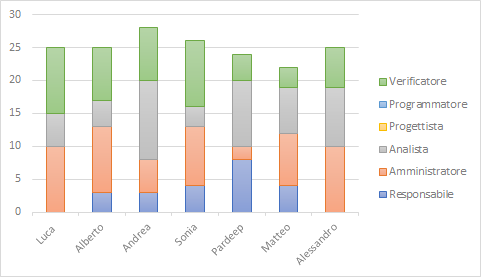
\includegraphics[width=15cm,keepaspectratio]{../includes/pics/grafici/grafico1.png}
	\caption{\label{fig:mission}Divisione dei ruoli tra i membri}
\end{figure}
\clearpage
\subsubsection{Prospetto economico}
Durante il periodo di analisi la distribuzione dei ruoli fra i membri del gruppo è stata la seguente:
\begin{center}
	\renewcommand{\arraystretch}{1.5}
	\rowcolors{3}{tableLightYellow}{}
	\begin{longtable}[H]{  	>{\RaggedRight}p{5.6cm}  
							>{\RaggedRight}p{3cm} 
							>{\RaggedRight}p{3cm}  
							}
		\rowcolor{tableHeadYellow}
		\textbf{Ruolo}   & \textbf{Ore} & \textbf{Costo (Euro)} \\ 
		\endhead
		Responsabile   & 22   & 660,00 \euro \\
		Amministratore & 54   & 1.080,00 \euro \\
		Analista       & 50   & 1.250,00 \euro\\
		Progettista    & 0    & 0,00 \euro \\
		Programmatore  & 0    & 0,00 \euro \\
		Verificatore   & 49   & 735,00 \euro\\
		Totale         & 175   & 3.725,00 \euro \\
		\rowcolor{white}
		\caption{Tabella prospetto economico}
	\end{longtable}
\end{center}
Il seguente grafico mostra visivamente la distribuzione dei ruoli:
%(immagine grafico 2)
\begin{figure}[H]
	\centering
	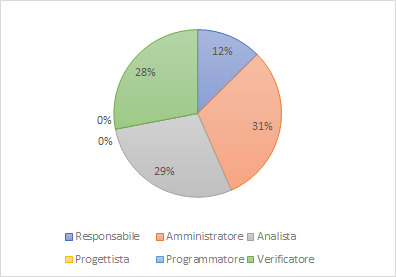
\includegraphics[width=15cm,keepaspectratio]{../includes/pics/grafici/grafico2.png}
	\caption{\label{fig:mission}Distribuzione oraria dei ruoli}
\end{figure}
\clearpage
\subsection{Consolidamento dei requisiti}
\label{sec:consolidamento_requisiti}
\subsubsection{Prospetto orario}
Durante il periodo di consolidamento la distribuzione oraria fra i membri del gruppo è stata la seguente:
\begin{center}
	\renewcommand{\arraystretch}{1.5}
	\rowcolors{3}{tableLightYellow}{}
	\begin{longtable}[H]{ 	>{\RaggedRight}p{3.5cm}  
							>{\Centering}p{1.2cm} 
							>{\Centering}p{1.2cm}  
							>{\Centering}p{1.2cm} 
							>{\Centering}p{1.2cm}  
							>{\Centering}p{1.2cm} 
							>{\Centering}p{1.2cm}  
							>{\Centering}p{1.4cm}  
							}
		\rowcolor{tableHeadYellow}
		\textbf{Nome}   & \textbf{Re} & \textbf{Ad} & \textbf{An} & \textbf{Pj} & \textbf{Pr} & \textbf{Ve} & \textbf{TOT} \\ 
		\endhead
		
		Luca Stocco         & 6   & 1     & 0   & 0   & 0   & 0  & 7 \\  
		Alberto Miola       & 0   & 2     & 0   & 0   & 0   & 5  & 7 \\  
		Andrea Pavin        & 0   & 0     & 4   & 0   & 0   & 3  & 7 \\  
		Sonia Menon         & 0   & 5     & 2   & 0   & 0   & 0  & 7 \\  
		Pardeep Singh       & 0   & 0     & 0   & 0   & 0   & 7  & 7 \\  
		Matteo Pellanda     & 0   & 0     & 7   & 0   & 0   & 0  & 7 \\
		Alessandro Pegoraro & 0   & 2 	  & 3   & 0	  & 0	& 2  & 7 \\ 

		\rowcolor{white}
		\caption{Tabella prospetto orario}
	\end{longtable}
\end{center}
Il seguente grafico mostra visivamente la distribuzione dei ruoli:
%(immagine grafico 3)
\begin{figure}[H]
	\centering
	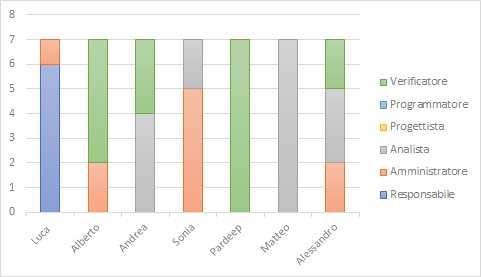
\includegraphics[width=15cm,keepaspectratio]{../includes/pics/grafici/grafico3.png}
	\caption{\label{fig:mission}Divisione dei ruoli tra i membri}
\end{figure}
\clearpage
\subsubsection{Prospetto economico}
Durante il periodo di consolidamento la distribuzione dei ruoli fra i membri del gruppo è stata la seguente:
\begin{center}
	\renewcommand{\arraystretch}{1.5}
	\rowcolors{3}{tableLightYellow}{}
	\begin{longtable}[H]{  	>{\RaggedRight}p{5.6cm}  
							>{\RaggedRight}p{3cm} 
							>{\RaggedRight}p{3cm}  
							}
		\rowcolor{tableHeadYellow}
		\textbf{Ruolo}   & \textbf{Ore} & \textbf{Costo (Euro)} \\ 
		\endhead

		Responsabile   & 6    & 180,00 \\
		Amministratore & 10    & 160,00 \\
		Analista       & 16   & 325,00 \\
		Progettista    & 0    & 0,00 \\
		Programmatore  & 0    & 0,00 \\
		Verificatore   & 17   & 225,00 \\
		Totale         & 49   & 890,00 \\

		\rowcolor{white}
		\caption{Tabella prospetto economico}
	\end{longtable}
\end{center}
Il seguente grafico mostra visivamente la distribuzione dei ruoli:
%(immagine grafico 4)
\begin{figure}[H]
	\centering
	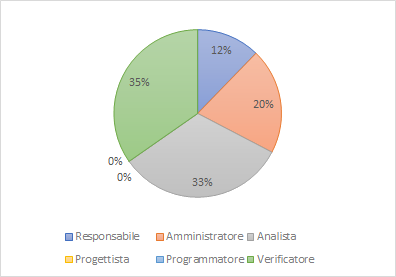
\includegraphics[width=15cm,keepaspectratio]{../includes/pics/grafici/grafico4.png}
	\caption{\label{fig:mission}Divisione dei ruoli tra i membri}
\end{figure}
\clearpage
\subsection{Technology Baseline}
\label{sec:technology_baseline}
\subsubsection{Prospetto orario}
Durante il periodo di technology baseline la distribuzione oraria fra i membri del gruppo è stata la seguente:
\begin{center}
	\renewcommand{\arraystretch}{1.5}
	\rowcolors{3}{tableLightYellow}{}
	\begin{longtable}[H]{ 	>{\RaggedRight}p{3.5cm}  
							>{\Centering}p{1.2cm} 
							>{\Centering}p{1.2cm}  
							>{\Centering}p{1.2cm} 
							>{\Centering}p{1.2cm}  
							>{\Centering}p{1.2cm} 
							>{\Centering}p{1.2cm}  
							>{\Centering}p{1.4cm}  
							}
		\rowcolor{tableHeadYellow}
		\textbf{Nome}   & \textbf{Re} & \textbf{Ad} & \textbf{An} & \textbf{Pj} & \textbf{Pr} & \textbf{Ve} & \textbf{TOT} \\ 
		\endhead

		Luca Stocco         & 4   & 0     & 0 	& 6		& 0 	& 3  	& 13 \\  
		Alberto Miola       & 0   & 0     & 2  	& 8  	& 0   	& 1  	& 11 \\  
		Andrea Pavin        & 3   & 5     & 0   & 4  	& 0   	& 3  	& 15 \\  
		Sonia Menon         & 0   & 3     & 2   & 5   	& 0  	& 4 	& 14 \\  
		Pardeep Singh       & 0   & 1     & 0   & 9  	& 0  	& 2 	& 12 \\  
		Matteo Pellanda     & 1   & 0     & 1  	& 6   	& 0  	& 3  	& 11 \\ 
		Alessandro Pegoraro & 0   & 3	  & 1	& 7		& 0 	& 2 	& 13 \\  

		\rowcolor{white}
		\caption{Tabella prospetto orario}
	\end{longtable}
\end{center}
Il seguente grafico mostra visivamente la distribuzione dei ruoli:
%(immagine grafico 5)
\begin{figure}[H]
	\centering
	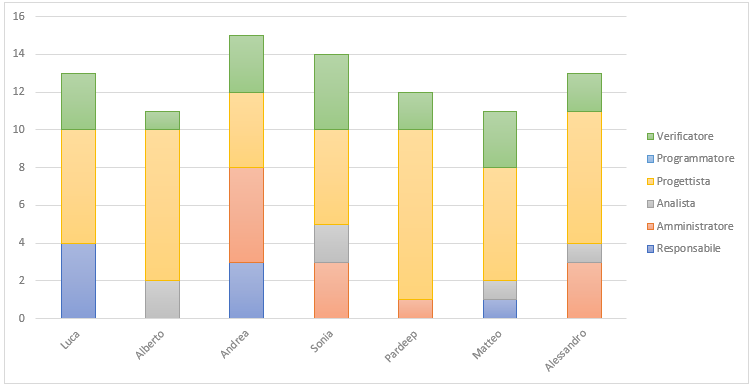
\includegraphics[width=15cm,keepaspectratio]{../includes/pics/grafici/tba.png}
	\caption{\label{fig:mission}Distribuzione oraria dei ruoli}
\end{figure}
\clearpage
\subsubsection{Prospetto economico}
Durante il periodo di technology baseline la distribuzione dei ruoli fra i membri del gruppo è stata la seguente:
\begin{center}
	\renewcommand{\arraystretch}{1.5}
	\rowcolors{3}{tableLightYellow}{}
	\begin{longtable}[H]{  	>{\RaggedRight}p{5.6cm}  
							>{\RaggedRight}p{3cm} 
							>{\RaggedRight}p{3cm}  
							}

		\rowcolor{tableHeadYellow}
		\textbf{Ruolo}   & \textbf{Ore} & \textbf{Costo (Euro)} \\ 
		\endhead

		Responsabile   & 8   & 240,00 \\
		Amministratore & 12   & 240,00 \\
		Analista       & 6   & 150,00 \\
		Progettista    & 45   & 990,00 \\
		Programmatore  & 0  & 0,00 \\
		Verificatore   & 18   & 270,00 \\
		Totale         & 89  & 1.890,00 \\

		\rowcolor{white}
		\caption{Tabella prospetto economico}
	\end{longtable}
\end{center}
Il seguente grafico mostra visivamente la distribuzione dei ruoli:
%(immagine grafico 6)
\begin{figure}[H]
	\centering
	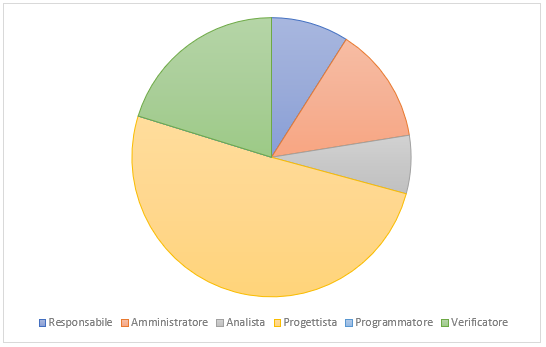
\includegraphics[width=15cm,keepaspectratio]{../includes/pics/grafici/tbb.png}
	\caption{\label{fig:mission}Divisione dei ruoli tra i membri}
\end{figure}
\clearpage
\subsection{Sprint 1}
\label{sec:sprint_1}
\subsubsection{Prospetto orario}
Durante il periodo del primo sprint la distribuzione oraria fra i membri del gruppo è stata la seguente:
\begin{center}
	\renewcommand{\arraystretch}{1.5}
	\rowcolors{3}{tableLightYellow}{}
	\begin{longtable}[H]{ 	>{\RaggedRight}p{3.5cm}  
							>{\Centering}p{1.2cm} 
							>{\Centering}p{1.2cm}  
							>{\Centering}p{1.2cm} 
							>{\Centering}p{1.2cm}  
							>{\Centering}p{1.2cm} 
							>{\Centering}p{1.2cm}  
							>{\Centering}p{1.4cm}  
							}
							
		\rowcolor{tableHeadYellow}
		\textbf{Nome}   & \textbf{Re} & \textbf{Ad} & \textbf{An} & \textbf{Pj} & \textbf{Pr} & \textbf{Ve} & \textbf{TOT} \\ 
		\endhead

		Luca Stocco         & 3   & 0     & 2   & 2   & 4   & 9   	& 20 \\  
		Alberto Miola       & 0   & 0     & 2   & 0   & 12  & 4  	& 18 \\  
		Andrea Pavin        & 3   & 2     & 0   & 2   & 5   & 7  	& 19 \\  
		Sonia Menon         & 0   & 1     & 0   & 1   & 8   & 7 	& 17 \\  
		Pardeep Singh       & 0   & 2     & 0   & 1   & 4   & 8  	& 15 \\  
		Matteo Pellanda     & 2   & 0     & 1   & 0   & 7   & 6 	& 16 \\
		Alessandro Pegoraro & 0   & 1	  & 2	& 0   & 6	& 5 	& 14 \\   

		\rowcolor{white}
		\caption{Tabella prospetto orario}
	\end{longtable}
\end{center}
Il seguente grafico mostra visivamente la distribuzione dei ruoli:
%(immagine grafico 7)
\begin{figure}[H]
	\centering
	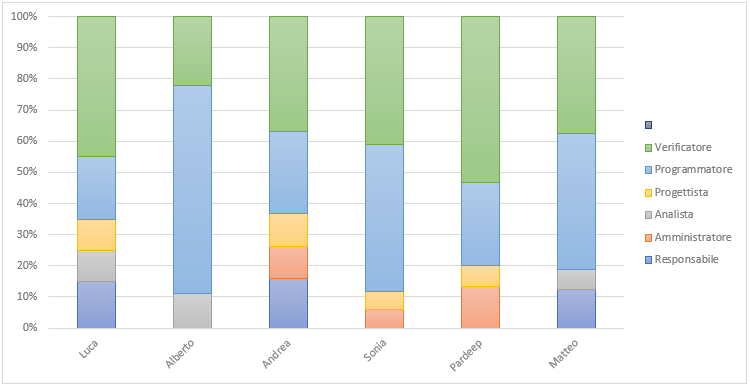
\includegraphics[width=15cm,keepaspectratio]{../includes/pics/grafici/sprint1a.png}
	\caption{\label{fig:mission}Distribuzione oraria dei ruoli}
\end{figure}
\clearpage
\subsubsection{Prospetto economico}
Durante il periodo del primo sprint la distribuzione dei ruoli fra i membri del gruppo è stata la seguente:
\begin{center}
	\renewcommand{\arraystretch}{1.5}
	\rowcolors{3}{tableLightYellow}{}
	\begin{longtable}[H]{  	>{\RaggedRight}p{5.6cm}  
							>{\RaggedRight}p{3cm} 
							>{\RaggedRight}p{3cm}  
							}

		\rowcolor{tableHeadYellow}
		\textbf{Ruolo}   & \textbf{Ore} & \textbf{Costo (Euro)} \\ 
		\endhead

		Responsabile   & 8   & 240,00 \\
		Amministratore & 6   & 120,00 \\
		Analista       & 7   & 175,00 \\
		Progettista    & 6   & 132,00 \\
		Programmatore  & 46  & 690,00 \\
		Verificatore   & 46  & 690,00 \\
		Totale         & 119 & 2.047,00 \\

		\rowcolor{white}
		\caption{Tabella prospetto economico}
	\end{longtable}
\end{center}
Il seguente grafico mostra visivamente la distribuzione dei ruoli:
%(immagine grafico 8)
\begin{figure}[H]
	\centering
	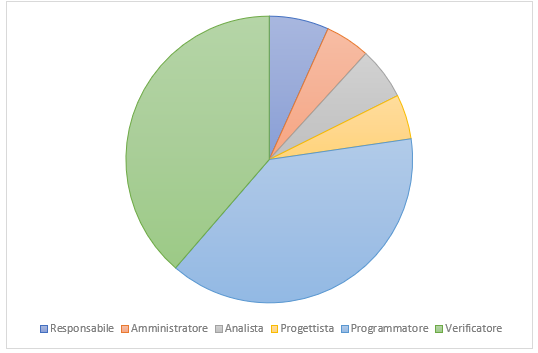
\includegraphics[width=15cm,keepaspectratio]{../includes/pics/grafici/sprint1b.png}
	\caption{\label{fig:mission}Divisione dei ruoli tra i membri}
\end{figure}
\clearpage
\subsection{Sprint 2}
\label{sec:sprint_2}
\subsubsection{Prospetto orario}
Durante il periodo del secondo sprint la distribuzione oraria fra i membri del gruppo è stata la seguente:
\begin{center}
	\renewcommand{\arraystretch}{1.5}
	\rowcolors{3}{tableLightYellow}{}
	\begin{longtable}[H]{ 	>{\RaggedRight}p{3.5cm}  
							>{\Centering}p{1.2cm} 
							>{\Centering}p{1.2cm}  
							>{\Centering}p{1.2cm} 
							>{\Centering}p{1.2cm}  
							>{\Centering}p{1.2cm} 
							>{\Centering}p{1.2cm}  
							>{\Centering}p{1.4cm}  
							}
							
		\rowcolor{tableHeadYellow}
		\textbf{Nome}   & \textbf{Re} & \textbf{Ad} & \textbf{An} & \textbf{Pj} & \textbf{Pr} & \textbf{Ve} & \textbf{TOT} \\ 
		\endhead

		Luca Stocco         & 0   & 2     & 0   & 9   & 5   & 3   	& 19 \\  
		Alberto Miola       & 2   & 2     & 0   & 7   & 6   & 5  	& 22 \\  
		Andrea Pavin        & 0   & 0     & 2   & 9   & 7   & 6  	& 24 \\  
		Sonia Menon         & 0   & 0     & 0   & 8   & 8   & 7 	& 23 \\  
		Pardeep Singh       & 1   & 2     & 3   & 9   & 7   & 5  	& 27 \\  
		Matteo Pellanda     & 0   & 1     & 2   & 7   & 6   & 4 	& 20 \\
		Alessandro Pegoraro & 3   & 1	  & 2	& 10  & 6	& 4 	& 26 \\   

		\rowcolor{white}
		\caption{Tabella prospetto orario}
	\end{longtable}
\end{center}
Il seguente grafico mostra visivamente la distribuzione dei ruoli:
%(immagine grafico 7)
\begin{figure}[H]
	\centering
	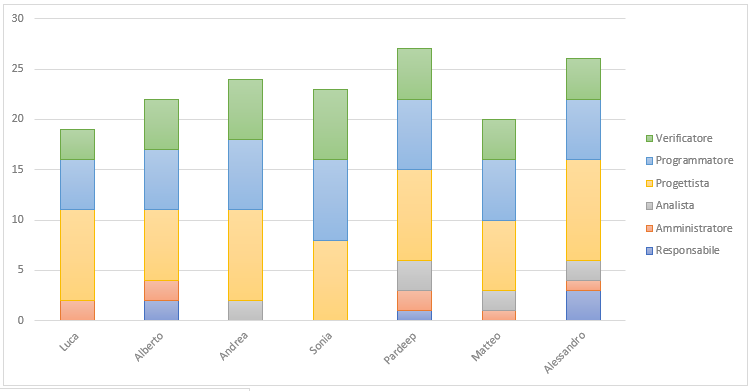
\includegraphics[width=15cm,keepaspectratio]{../includes/pics/grafici/sprint2a.png}
	\caption{\label{fig:mission}Distribuzione oraria dei ruoli}
\end{figure}
\clearpage
\subsubsection{Prospetto economico}
Durante il periodo del secondo sprint la distribuzione dei ruoli fra i membri del gruppo è stata la seguente:
\begin{center}
	\renewcommand{\arraystretch}{1.5}
	\rowcolors{3}{tableLightYellow}{}
	\begin{longtable}[H]{  	>{\RaggedRight}p{5.6cm}  
							>{\RaggedRight}p{3cm} 
							>{\RaggedRight}p{3cm}  
							}

		\rowcolor{tableHeadYellow}
		\textbf{Ruolo}   & \textbf{Ore} & \textbf{Costo (Euro)} \\ 
		\endhead

		Responsabile   & 6   & 180,00 \\
		Amministratore & 8   & 160,00 \\
		Analista       & 9   & 225,00 \\
		Progettista    & 59  & 1.298,00 \\
		Programmatore  & 45  & 675,00 \\
		Verificatore   & 34  & 510,00 \\
		Totale         & 161 & 3.048,00 \\

		\rowcolor{white}
		\caption{Tabella prospetto economico}
	\end{longtable}
\end{center}
Il seguente grafico mostra visivamente la distribuzione dei ruoli:
%(immagine grafico 8)
\begin{figure}[H]
	\centering
	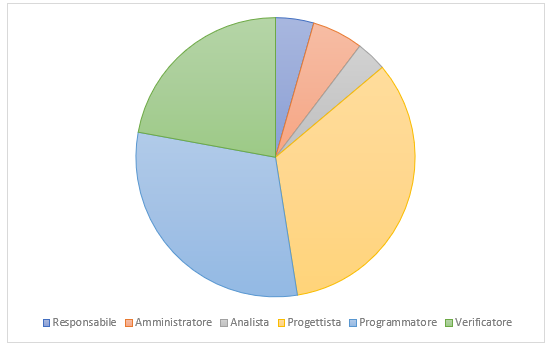
\includegraphics[width=15cm,keepaspectratio]{../includes/pics/grafici/sprint2b.png}
	\caption{\label{fig:mission}Divisione dei ruoli tra i membri}
\end{figure}
\clearpage
\subsection{Sprint 3}
\label{sec:sprint_3}
\subsubsection{Prospetto orario}
Durante il periodo del terzo sprint la distribuzione oraria fra i membri del gruppo è stata la seguente:
\begin{center}
	\renewcommand{\arraystretch}{1.5}
	\rowcolors{3}{tableLightYellow}{}
	\begin{longtable}[H]{ 	>{\RaggedRight}p{3.5cm}  
							>{\Centering}p{1.2cm} 
							>{\Centering}p{1.2cm}  
							>{\Centering}p{1.2cm} 
							>{\Centering}p{1.2cm}  
							>{\Centering}p{1.2cm} 
							>{\Centering}p{1.2cm}  
							>{\Centering}p{1.4cm}  
							}
							
		\rowcolor{tableHeadYellow}
		\textbf{Nome}   & \textbf{Re} & \textbf{Ad} & \textbf{An} & \textbf{Pj} & \textbf{Pr} & \textbf{Ve} & \textbf{TOT} \\ 
		\endhead

		Luca Stocco         & 0	& 2 & 0 & 7  & 12 & 3 & 24 \\  
		Alberto Miola       & 3	& 3	& 0	& 8	 & 5  & 8 & 27 \\  
		Andrea Pavin        & 0	& 0	& 1	& 7	 & 10 & 4 & 23 \\  
		Sonia Menon         & 0	& 0	& 0	& 8	 & 8  & 5 & 21 \\  
		Pardeep Singh       & 2	& 2	& 1	& 11 & 12 & 6 & 34 \\  
		Matteo Pellanda     & 0	& 3	& 1	& 11 & 8  & 6 & 29 \\
		Alessandro Pegoraro & 4	& 2	& 0	& 7	 & 7  & 7 & 27 \\   

		\rowcolor{white}
		\caption{Tabella prospetto orario}
	\end{longtable}
\end{center}
Il seguente grafico mostra visivamente la distribuzione dei ruoli:
%(immagine grafico 7)
\begin{figure}[H]
	\centering
	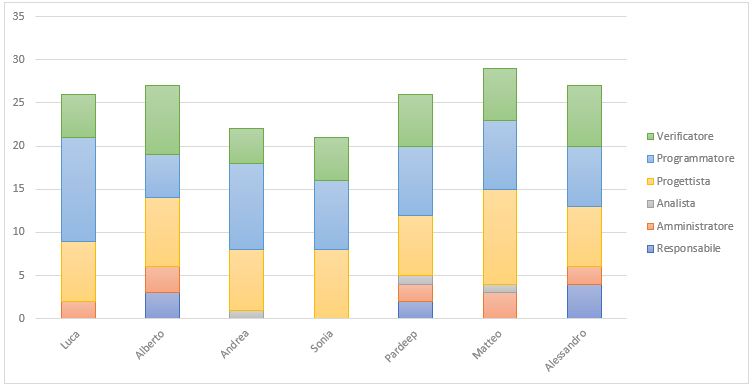
\includegraphics[width=15cm,keepaspectratio]{../includes/pics/grafici/sprint3a.png}
	\caption{\label{fig:mission}Distribuzione oraria dei ruoli}
\end{figure}
\clearpage
\subsubsection{Prospetto economico}
Durante il periodo del terzo sprint la distribuzione dei ruoli fra i membri del gruppo è stata la seguente:
\begin{center}
	\renewcommand{\arraystretch}{1.5}
	\rowcolors{3}{tableLightYellow}{}
	\begin{longtable}[H]{  	>{\RaggedRight}p{5.6cm}  
							>{\RaggedRight}p{3cm} 
							>{\RaggedRight}p{3cm}  
							}

		\rowcolor{tableHeadYellow}
		\textbf{Ruolo}   & \textbf{Ore} & \textbf{Costo (Euro)} \\ 
		\endhead

		Responsabile   & 9   & 270,00 \\
		Amministratore & 12  & 240,00 \\
		Analista       & 4   & 75,00 \\
		Progettista    & 59  & 1.298,00 \\
		Programmatore  & 62  & 930,00 \\
		Verificatore   & 39  & 585,00 \\
		Totale         & 178 & 3.398,00 \\

		\rowcolor{white}
		\caption{Tabella prospetto economico}
	\end{longtable}
\end{center}
Il seguente grafico mostra visivamente la distribuzione dei ruoli:
%(immagine grafico 8)
\begin{figure}[H]
	\centering
	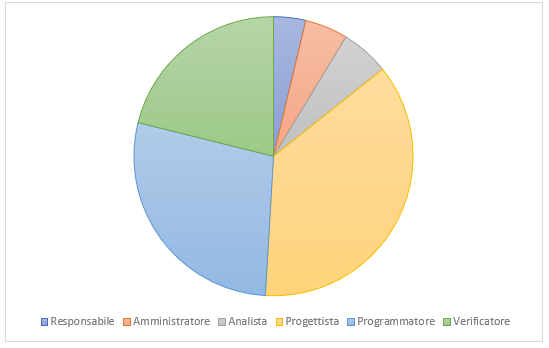
\includegraphics[width=15cm,keepaspectratio]{../includes/pics/grafici/sprint3b.png}
	\caption{\label{fig:mission}Divisione dei ruoli tra i membri}
\end{figure}
\clearpage
\subsection{Sprint 4}
\label{sec:sprint_4}
\subsubsection{Prospetto orario}
Durante il periodo del quarto sprint la distribuzione oraria fra i membri del gruppo è stata la seguente:
\begin{center}
	\renewcommand{\arraystretch}{1.5}
	\rowcolors{3}{tableLightYellow}{}
	\begin{longtable}[H]{ 	>{\RaggedRight}p{3.5cm}  
							>{\Centering}p{1.2cm} 
							>{\Centering}p{1.2cm}  
							>{\Centering}p{1.2cm} 
							>{\Centering}p{1.2cm}  
							>{\Centering}p{1.2cm} 
							>{\Centering}p{1.2cm}  
							>{\Centering}p{1.4cm}  
							}
							
		\rowcolor{tableHeadYellow}
		\textbf{Nome}   & \textbf{Re} & \textbf{Ad} & \textbf{An} & \textbf{Pj} & \textbf{Pr} & \textbf{Ve} & \textbf{TOT} \\ 
		\endhead

		Luca Stocco         & 0	& 2 & 0 & 3  & 3  & 3 & 11 \\  		
		Alberto Miola       & 0	& 2	& 0	& 4	 & 2  & 3 & 11 \\  		
		Andrea Pavin        & 0	& 1	& 0	& 3	 & 2  & 3 & 9 \\  		
		Sonia Menon         & 5	& 1	& 0	& 3	 & 1  & 1 & 11 \\ 
		Pardeep Singh       & 0	& 0	& 0	& 0  & 4  & 3 & 7 \\ 		 
		Matteo Pellanda     & 1	& 2	& 0	& 5  & 3  & 2 & 13 \\		
		Alessandro Pegoraro & 0	& 0	& 0	& 3	 & 4  & 3 & 10 \\ 
		
		\rowcolor{white}
		\caption{Tabella prospetto orario}
	\end{longtable}
\end{center}
Il seguente grafico mostra visivamente la distribuzione dei ruoli:
%(immagine grafico 7)
\begin{figure}[H]
	\centering
	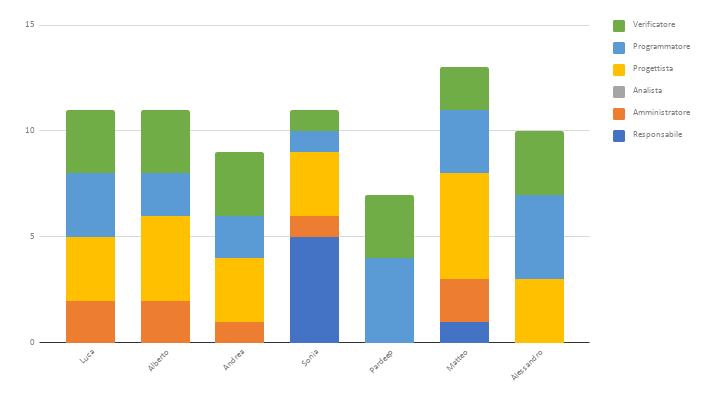
\includegraphics[width=15cm,keepaspectratio]{../includes/pics/grafici/sprint4a.png}
	\caption{\label{fig:mission}Distribuzione oraria dei ruoli}
\end{figure}
\clearpage
\subsubsection{Prospetto economico}
Durante il periodo del quarto sprint la distribuzione dei ruoli fra i membri del gruppo è stata la seguente:
\begin{center}
	\renewcommand{\arraystretch}{1.5}
	\rowcolors{3}{tableLightYellow}{}
	\begin{longtable}[H]{  	>{\RaggedRight}p{5.6cm}  
							>{\RaggedRight}p{3cm} 
							>{\RaggedRight}p{3cm}  
							}

		\rowcolor{tableHeadYellow}
		\textbf{Ruolo}   & \textbf{Ore} & \textbf{Costo (Euro)} \\ 
		\endhead

		Responsabile   & 6   & 180,00 \\
		Amministratore & 8   & 160,00 \\
		Analista       & 0   & 0,00 \\
		Progettista    & 21  & 462,00 \\
		Programmatore  & 19  & 285,00 \\
		Verificatore   & 18  & 270,00 \\
		Totale         & 72  & 1.357,00 \\

		\rowcolor{white}
		\caption{Tabella prospetto economico}
	\end{longtable}
\end{center}
Il seguente grafico mostra visivamente la distribuzione dei ruoli:
%(immagine grafico 8)
\begin{figure}[H]
	\centering
	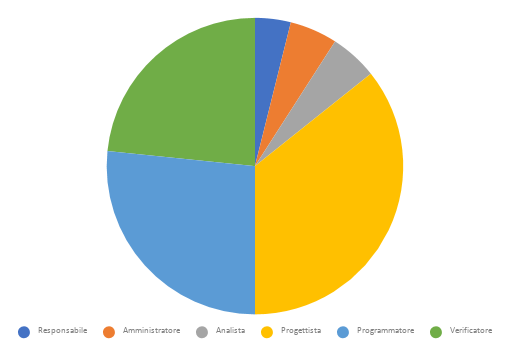
\includegraphics[width=15cm,keepaspectratio]{../includes/pics/grafici/sprint4b.png}
	\caption{\label{fig:mission}Divisione dei ruoli tra i membri}
\end{figure}
\clearpage
\subsection{Sprint 5}
\label{sec:sprint_5}
\subsubsection{Prospetto orario}
Durante il periodo del quinto sprint la distribuzione oraria fra i membri del gruppo è stata la seguente:
\begin{center}
	\renewcommand{\arraystretch}{1.5}
	\rowcolors{3}{tableLightYellow}{}
	\begin{longtable}[H]{ 	>{\RaggedRight}p{3.5cm}  
							>{\Centering}p{1.2cm} 
							>{\Centering}p{1.2cm}  
							>{\Centering}p{1.2cm} 
							>{\Centering}p{1.2cm}  
							>{\Centering}p{1.2cm} 
							>{\Centering}p{1.2cm}  
							>{\Centering}p{1.4cm}  
							}
							
		\rowcolor{tableHeadYellow}
		\textbf{Nome}   & \textbf{Re} & \textbf{Ad} & \textbf{An} & \textbf{Pj} & \textbf{Pr} & \textbf{Ve} & \textbf{TOT} \\ 
		\endhead

		Luca Stocco         & 0	& 2 & 0 & 3  & 3  & 5 & 13 \\  		
		Alberto Miola       & 0	& 2	& 0	& 4	 & 2  & 3 & 11 \\  		
		Andrea Pavin        & 0	& 2	& 0	& 3	 & 3  & 3 & 11 \\  		
		Sonia Menon         & 4	& 2	& 0	& 3	 & 2  & 2 & 13 \\ 
		Pardeep Singh       & 1	& 0	& 0	& 0  & 1  & 2 & 4 \\ 		 
		Matteo Pellanda     & 1	& 3	& 0	& 0  & 3  & 3 & 10 \\		
		Alessandro Pegoraro & 0	& 0	& 0	& 2	 & 4  & 4 & 10 \\ 
		
		\rowcolor{white}
		\caption{Tabella prospetto orario}
	\end{longtable}
\end{center}
Il seguente grafico mostra visivamente la distribuzione dei ruoli:
%(immagine grafico 7)
\begin{figure}[H]
	\centering
	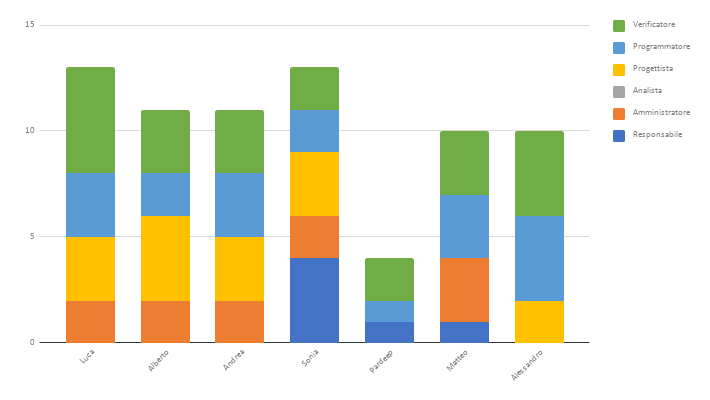
\includegraphics[width=15cm,keepaspectratio]{../includes/pics/grafici/sprint5a.png}
	\caption{\label{fig:mission}Distribuzione oraria dei ruoli}
\end{figure}
\clearpage
\subsubsection{Prospetto economico}
Durante il periodo del quinto sprint la distribuzione dei ruoli fra i membri del gruppo è stata la seguente:
\begin{center}
	\renewcommand{\arraystretch}{1.5}
	\rowcolors{3}{tableLightYellow}{}
	\begin{longtable}[H]{  	>{\RaggedRight}p{5.6cm}  
							>{\RaggedRight}p{3cm} 
							>{\RaggedRight}p{3cm}  
							}

		\rowcolor{tableHeadYellow}
		\textbf{Ruolo}   & \textbf{Ore} & \textbf{Costo (Euro)} \\ 
		\endhead

		Responsabile   & 6   & 180,00 \\
		Amministratore & 11  & 220,00 \\
		Analista       & 0   & 0,00 \\
		Progettista    & 15  & 330,00 \\
		Programmatore  & 18  & 270,00 \\
		Verificatore   & 22  & 330,00 \\
		Totale         & 74  & 1.330,00 \\

		\rowcolor{white}
		\caption{Tabella prospetto economico}
	\end{longtable}
\end{center}
Il seguente grafico mostra visivamente la distribuzione dei ruoli:
%(immagine grafico 8)
\begin{figure}[H]
	\centering
	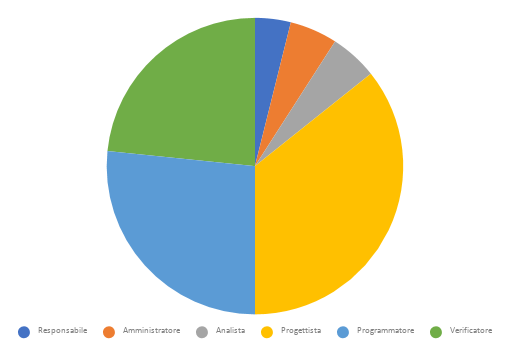
\includegraphics[width=15cm,keepaspectratio]{../includes/pics/grafici/sprint5b.png}
	\caption{\label{fig:mission}Divisione dei ruoli tra i membri}
\end{figure}
%\clearpage
%\subsection{Validazione e collaudo}
%\label{sec:validazione_collaudo}
%\subsubsection{Prospetto orario}
%Durante il periodo di validazione la distribuzione oraria fra i membri del gruppo è stata la seguente:
%\begin{center}
%	\renewcommand{\arraystretch}{1.5}
%	\rowcolors{3}{tableLightYellow}{}
%	\begin{longtable}[H]{ 	>{\RaggedRight}p{3.5cm}  
%							>{\Centering}p{1.2cm} 
%							>{\Centering}p{1.2cm}  
%							>{\Centering}p{1.2cm} 
%							>{\Centering}p{1.2cm}  
%							>{\Centering}p{1.2cm} 
%							>{\Centering}p{1.2cm}  
%							>{\Centering}p{1.4cm}  
%							}
%							
%		\rowcolor{tableHeadYellow}
%		\textbf{Nome}   & \textbf{Re} & \textbf{Ad} & \textbf{An} & \textbf{Pj} & \textbf{Pr} & \textbf{Ve} & \textbf{TOT} \\ 
%		\endhead
%
%		Luca Stocco       & 0   & 4     & 0   & 6    & 6    & 6   	& 22 \\  
%		Alberto Miola     & 0   & 4     & 0   & 8    & 4    & 6   	& 22 \\  
%		Andrea Pavin      & 0   & 3     & 0   & 6    & 5    & 6   	& 20 \\  
%		Sonia Menon       & 10  & 3     & 0   & 6    & 3    & 3   	& 25 \\  
%		Pardeep Singh     & 2   & 0     & 0   & 4    & 9    & 6   	& 21 \\  
%		Matteo Pellanda   & 3   & 5     & 0   & 5    & 6    & 5   	& 24 \\ 
%		Alessandro Pegoraro & 0 & 0		& 0	  & 5	 & 8 	& 7 	& 20 \\  
%
%		\rowcolor{white}
%		\caption{Tabella prospetto orario}
%	\end{longtable}
%\end{center}
%Il seguente grafico mostra visivamente la distribuzione dei ruoli:
%(immagine grafico 9)
%\begin{figure}[H]
%	\centering
%	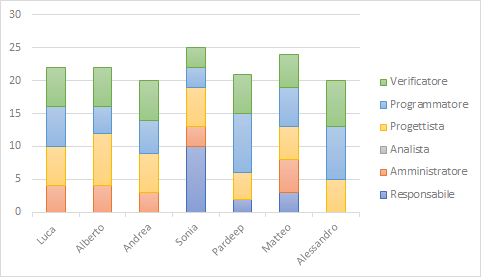
\includegraphics[width=15cm,keepaspectratio]{../includes/pics/grafici/grafico9.png}
%	\caption{\label{fig:mission}Distribuzione oraria dei ruoli}
%\end{figure}
%\clearpage
%\subsubsection{Prospetto economico}
%Durante il periodo di validazione la distribuzione dei ruoli fra i membri del gruppo è stata la seguente:
%\begin{center}
%	\renewcommand{\arraystretch}{1.5}
%	\rowcolors{3}{tableLightYellow}{}
%	\begin{longtable}[H]{  	>{\RaggedRight}p{5.6cm}  
%							>{\RaggedRight}p{3cm} 
%							>{\RaggedRight}p{3cm}  
%							}
%							
%		\rowcolor{tableHeadYellow}
%		\textbf{Ruolo}   & \textbf{Ore} & \textbf{Costo (Euro)} \\ 
%		\endhead
%
%		Responsabile   & 15   & 450,00 \\
%		Amministratore & 19   & 380,00 \\
%		Analista       & 0    & 0,00 \\
%		Progettista    & 40   & 880,00 \\
%		Programmatore  & 41   & 615,00 \\
%		Verificatore   & 39   & 585,00 \\
%		Totale         & 154  & 2.677,00 \\
%
%		\rowcolor{white}
%		\caption{Tabella prospetto economico}
%	\end{longtable}
%\end{center}
%Il seguente grafico mostra visivamente la distribuzione dei ruoli:
%(immagine grafico 10)
%\begin{figure}[H]
%	\centering
%	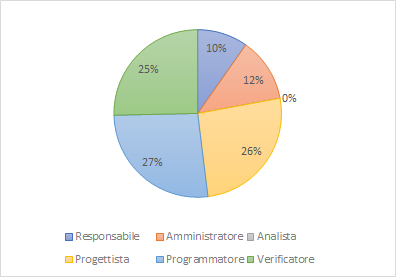
\includegraphics[width=15cm,keepaspectratio]{../includes/pics/grafici/grafico10.png}
%	\caption{\label{fig:mission}Divisione dei ruoli tra i membri}
%\end{figure}
\clearpage
\subsection{Totale ore rendicontate}
\label{sec:totale_ore}
\subsubsection{Totale suddivisione ore rendicontate}
Di seguito viene riportato il totale delle ore rendicontane nel preventivo finale a carico del committente:
\begin{center}
	\renewcommand{\arraystretch}{1.5}
	\rowcolors{3}{tableLightYellow}{}
	\begin{longtable}[H]{ 	>{\RaggedRight}p{3.5cm}  
							>{\Centering}p{1.2cm} 
							>{\Centering}p{1.2cm}  
							>{\Centering}p{1.2cm} 
							>{\Centering}p{1.2cm}  
							>{\Centering}p{1.2cm} 
							>{\Centering}p{1.2cm}  
							>{\Centering}p{1.4cm}  
							}
							
		\rowcolor{tableHeadYellow}
		\textbf{Nome}   & \textbf{Re} & \textbf{Ad} & \textbf{An} & \textbf{Pj} & \textbf{Pr} & \textbf{Ve} & \textbf{TOT} \\ 
		\endhead
 
		Luca Stocco         & 7   & 8     & 2   & 30   & 29    & 26   &   102 \\  
		Alberto Miola       & 5   & 10     & 4   & 30   & 27    & 24   &   100 \\  
		Andrea Pavin        & 6   & 10    & 3   & 28   & 28    & 26   &   101 \\  
		Sonia Menon         & 7  & 7     & 2   & 28   & 30    & 30    &   104 \\ %FALSISSIMA
		Pardeep Singh       & 4   & 7     & 4   & 30   & 30    & 26   &   101 \\  
		Matteo Pellanda     & 5   & 10     & 5   & 29   & 27    & 24   &   100 \\
		Alessandro Pegoraro & 7   & 7	  & 5	& 29   & 27    & 27   &   102\\   

		\rowcolor{white}
		\caption{Tabella suddivisione ore rendicontate}
	\end{longtable}
\end{center}
Il seguente grafico mostra visivamente la distribuzione dei ruoli:
%(immagine grafico 11)
\begin{figure}[H]
	\centering
	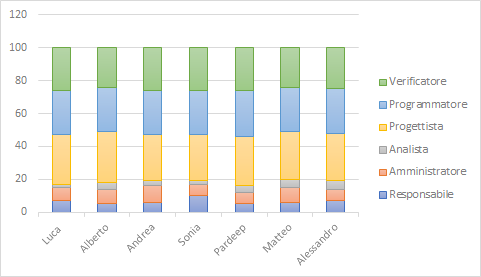
\includegraphics[width=15cm,keepaspectratio]{../includes/pics/grafici/grafico11.png}
	\caption{\label{fig:mission}Distribuzione oraria dei ruoli}
\end{figure}
\clearpage
\subsubsection{Totale prospetto economico rendicontato}
\begin{center}
	\renewcommand{\arraystretch}{1.5}
	\rowcolors{3}{tableLightYellow}{}
	\begin{longtable}[H]{  	>{\RaggedRight}p{5.6cm}  
							>{\RaggedRight}p{3cm} 
							>{\RaggedRight}p{3cm}  
							}

		\rowcolor{tableHeadYellow}
		\textbf{Ruolo}   & \textbf{Ore} & \textbf{Costo (Euro)} \\ 
		\endhead

		Responsabile   & 41    & 1.230,00 \\
		Amministratore & 59    & 1.180,00 \\
		Analista       & 25    & 625,00 \\
		Progettista    & 196   & 4.312,00 \\
		Programmatore  & 198   & 2.970,00 \\
		Verificatore   & 183   & 2.745,00 \\
		Totale         & 702   & 13.057,00 \\

		\rowcolor{white}
		\caption{Tabella prospetto economico rendicontato}
	\end{longtable}
\end{center}
Il seguente grafico mostra visivamente la distribuzione dei ruoli:
%(immagine grafico 12)
\begin{figure}[H]
	\centering
	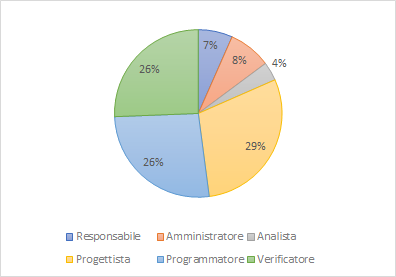
\includegraphics[width=15cm,keepaspectratio]{../includes/pics/grafici/grafico12.png}
	\caption{\label{fig:mission}Divisione dei ruoli tra i membri}
\end{figure}
